% ARCHIVED identity (FS-HSAC). Live paper is ../main.tex: Feasible-Support Hybrid TD3 (PC-HybridTD3).
\documentclass[conference]{IEEEtran}
\IEEEoverridecommandlockouts
\usepackage{cite}
\usepackage{amsmath,amssymb,amsfonts}
\usepackage{graphicx}
\usepackage{textcomp}
\usepackage{booktabs}
\usepackage{bm}
\usepackage{array}
\usepackage{algorithm}
\usepackage{algpseudocode}
\usepackage{placeins}
\usepackage{flushend}
\usepackage{url}
\urlstyle{same}
\graphicspath{{figures/}}

\begin{document}

\title{Feasible-Support Hybrid SAC for Weekly Dispatch\\of a Thermal--Battery--CAES Plant}

\author{
\IEEEauthorblockN{Anonymous Authors}
}

\maketitle

\begin{abstract}
This paper studies weekly price-taker dispatch of a thermal--battery--compressed-air energy storage (CAES) plant under Shandong's 2026 monthly 110\,kV agency-purchase time-of-use (TOU) tariff and a China National ETS carbon charge. The plant is a first-principles Modelica model of multi-tank adiabatic CAES with coupled gas and thermal dynamics, built in MWORKS Sysplorer and exported as an FMI functional mock-up unit (FMU). The CAES electric command occupies a disconnected envelope that shrinks further with mode locks and inventory, so the admissible action is a state-dependent hybrid set \(\mathcal{A}(s)\). We propose a feasible-support hybrid soft actor--critic (FS-HSAC) that places a same-hour policy density on this set and advances the twin only after a GiveSafe check. On three seasonal held-out weeks the controller completes all \(168\) hours, with a reject rate below \(0.4\%\) and no unserved energy. A rolling linear programme on the same FMU uses CAES, whereas the greedy FS-HSAC policy keeps CAES idle; both patterns are reported.
\end{abstract}

\begin{IEEEkeywords}
digital twin, compressed-air energy storage, hybrid-action reinforcement learning, Modelica, time-of-use
\end{IEEEkeywords}

\section{Introduction}

Weekly price-taker operation of a thermal--battery--CAES plant must settle Shandong's 2026 monthly 110\,kV agency-purchase TOU~\cite{shandong2026tou} and a National ETS carbon charge~\cite{mee2025etsnews}. The command is mixed: a thermal load rate, a battery power, a CAES mode in \(\{\mathrm{discharge},\mathrm{idle},\mathrm{charge}\}\), and a magnitude that belongs to that mode. The plant used here is a multi-tank adiabatic CAES Modelica model with coupled gas and thermal DAEs, built in MWORKS Sysplorer and stepped once per hour as an FMI FMU. On that twin the CAES electric command occupies a disconnected envelope, then shrinks further with mode locks and inventory. Sampling a box and projecting afterwards can turn a legal charge or discharge into idle, and unconstrained trial-and-error on the FMU is unsafe.

A multi-mode CAES--battery hub has been scheduled with option-based hierarchical RL~\cite{cui2024caesbess}. An initiation set of that kind can restrict when a mode may start; it does not define a same-hour density over three modes and the magnitude interval attached to each mode. Parameterized-action actor--critics already factor a discrete choice and a continuous parameter~\cite{fan2019hybrid}. This paper puts that factorisation on the state-dependent support that the twin can execute:
\begin{equation}
\mathcal{A}(s)
=
\mathcal{A}_{\mathrm{tp}}(s)\times
\mathcal{A}_{\mathrm{bat}}(s)\times
\bigcup_{k\in\mathcal{K}(s)}
\bigl(\{k\}\times\mathcal{M}_k(s)\bigr),
\label{eq:support}
\end{equation}
where \(\mathcal{K}(s)\subseteq\{\mathrm{dis},\mathrm{idle},\mathrm{chg}\}\) is the set of currently legal modes and \(\mathcal{M}_k(s)\) is the magnitude interval of mode \(k\).

FS-HSAC is a hybrid SAC on~\eqref{eq:support}: illegal modes have probability zero, and magnitude is mapped through \(\mathcal{M}_k(s)\) with a Jacobian correction of \(\log\pi\). GiveSafe is the last check before the FMU steps. The weekly objective \(J^{\mathrm{gen}}\) uses monthly 110\,kV cash, intensity-benchmark ETS, spill and unserved penalties, battery wear, CAES start-up and a soft interchange band; week-end inventory enters only as a terminal bonus. Section~\ref{sec:exp} reports three seasonal held-out weeks. The greedy policy keeps CAES idle, while a rolling linear programme on the same FMU uses CAES.

Section~\ref{sec:plant} describes the plant and the tariff. Section~\ref{sec:problem} states the weekly dispatch problem. Section~\ref{sec:method} presents FS-HSAC. Section~\ref{sec:exp} is the case study, and Section~\ref{sec:conclusion} concludes.

\section{Plant and Market}
\label{sec:plant}

Fig.~\ref{fig:topology} shows the plant. Wind, PV and the grid set the boundary. A thermal unit commanded by \(u_{\mathrm{tp}}\), a battery commanded by \(u_{\mathrm{bat}}\) and a multi-tank adiabatic CAES train share the electric bus. The Modelica model includes thermal ramping and fuel use, battery SoC with round-trip efficiency, CAES gas and hot/cold inventories, and nodal balance with curtailment and unserved residual. CAES has three tanks (gas, hot, cold) and switches among charge, idle and discharge. Agents interact with the exported FMU once per hour. The compiled FMU is the plant seen by the dispatcher.

\begin{figure}[!t]
\centering

\includegraphics[width=\columnwidth]{fig_topology}
\caption{Thermal--battery--CAES plant. The Modelica model is built in Sysplorer and exported as an FMI FMU.}
\label{fig:topology}
\end{figure}

Table~\ref{tab:params} lists the ratings used in the case study. Thermal power is \(P_t^{\mathrm{th}}=u_{\mathrm{tp},t}P_{\mathrm{cap}}^{\mathrm{th}}\) with \(u_{\mathrm{tp}}\in[1/3,1]\) (no shut-down) and a ramp limit of \(0.15\)\,p.u.\ per hour. Battery power is \(P_t^{\mathrm{bat}}=u_{\mathrm{bat},t}P_{\mathrm{cap}}^{\mathrm{bat}}\) on a \(100\)\,MW/\(500\)\,MWh unit with discharge efficiency \(0.85\) and SoC box \([0.1,0.9]\). CAES electric power on a \(150\)\,MW rating occupies the disconnected envelope
\begin{equation}
u_{\mathrm{caes}}
\in
[-1,-0.33]\;\cup\;\{0\}\;\cup\;[0.86,1],
\label{eq:legal}
\end{equation}
which encodes minimum compressor and expander loading. Mode locks and inventory margins shrink the set further. A hybrid action is \(a=(u_{\mathrm{tp}},u_{\mathrm{bat}},k,\mu)\). Magnitude \(\mu\in[0,1]\) is mapped through the current interval \(\mathcal{M}_k(s)\); idle has no magnitude. Equation~\eqref{eq:legal} is a plant constraint.

\begin{table}[!t]
\caption{Plant and market parameters.}
\label{tab:params}
\centering
\scriptsize
\setlength{\tabcolsep}{3.5pt}
\begin{tabular}{@{}lll@{}}
\toprule
Quantity & Value & Note \\
\midrule
Wind / PV nameplate & 300 / 260 MW & Resource-limited \\
Thermal \(P_{\min}\)--\(P_{\mathrm{cap}}\) & 50--150 MW & \(u_{\mathrm{tp}}\in[1/3,1]\); no shut-down \\
Battery power / energy & 100 MW / 500 MWh & \(\eta=0.85\) on discharge \\
CAES electric rating & 150 MW & Envelope~\eqref{eq:legal} \\
Grid hard / contract limits & \(\pm500\) / \(\pm200\) MW & Soft band priced in \(J^{\mathrm{gen}}\) \\
TOU sell & 0.1875 CNY/kWh & Flat export (scenario value) \\
ETS price \(\pi\) & 97.49 CNY/t & 2024 year-end CEA close \\
Curtailment / unserved & 300 / 1000 CNY/MWh & Objective penalties \\
Episode length \(T\) & 168 h & Weekly MDP \\
\bottomrule
\end{tabular}
\end{table}

The plant is a price-taker. Band windows and float ratios follow Shandong DRC Price [2023] No.~914 (peak \(+70\%\), valley \(-70\%\), sharp-peak \(+100\%\), deep-valley \(-90\%\))~\cite{shandong2023tou}. Absolute buy levels are taken from the 2026 monthly 110\,kV two-part delivered energy tables~\cite{shandong2026tou}, not from a year-constant five-tuple. Table~\ref{tab:tou} transcribes January--August (official); September--December carry the last published month. The two-part 110\,kV T\&D energy charge is \(0.1191\)\,CNY/kWh through July and \(0.106\)\,CNY/kWh from 1 August 2026. Fig.~\ref{fig:price} shows a winter held-out day and the January versus August clocks. Fig.~\ref{fig:boundary} shows weekly wind, irradiance, load and TOU on the three held-out windows (February, May and August on the 2026 calendar). The flat sell price \(0.1875\)\,CNY/kWh is a scenario value.

\begin{table}[!t]
\caption{2026 Shandong 110\,kV two-part agency-purchase TOU (CNY/kWh). O: official monthly table; S: August carried forward.}
\label{tab:tou}
\centering
\scriptsize
\begin{tabular}{@{}crrrrrrc@{}}
\toprule
Mo. & Sharp & Peak & Flat & Valley & Deep & T\&D & \\
\midrule
1 & 1.1873 & 1.0257 & 0.6488 & 0.2720 & 0.1643 & 0.1191 & O \\
2 & 1.1479 & 0.9936 & 0.6330 & 0.2726 & 0.1696 & 0.1191 & O \\
3 & 1.0648 & 0.9206 & 0.5841 & 0.2477 & 0.1515 & 0.1191 & O \\
4 & 1.0759 & 0.9275 & 0.5811 & 0.2349 & 0.1359 & 0.1191 & O \\
5 & 1.0489 & 0.9090 & 0.5824 & 0.2559 & 0.1626 & 0.1191 & O \\
6 & 1.0303 & 0.8946 & 0.5776 & 0.2608 & 0.1703 & 0.1191 & O \\
7 & 1.1037 & 0.9584 & 0.6190 & 0.2797 & 0.1827 & 0.1191 & O \\
8 & 1.0180 & 0.8844 & 0.5727 & 0.2611 & 0.1720 & 0.1060 & O \\
9--12 & 1.0180 & 0.8844 & 0.5727 & 0.2611 & 0.1720 & 0.1060 & S \\
\bottomrule
\end{tabular}
\end{table}

\begin{figure}[!t]
\centering

\includegraphics[width=\columnwidth]{fig_price_tou}
\caption{Purchase TOU on the monthly 110\,kV path. (a)~First day of the winter held-out week. (b)~January versus August on the same 24\,h clock.}
\label{fig:price}
\end{figure}

\begin{figure*}[!t]
\centering

\includegraphics[width=0.92\textwidth,height=6.4cm,keepaspectratio]{fig_seasonal_boundary}
\caption{Weekly wind speed, irradiance, electric load and monthly 110\,kV TOU purchase price on the three held-out weeks (winter week~5 / February, transition week~18 / May, summer week~31 / August).}
\label{fig:boundary}
\end{figure*}

\section{Weekly Dispatch Problem}
\label{sec:problem}

Let \(t=0,\ldots,T-1\) with \(T=168\). Grid purchase and sale energies are \(E_t^{\mathrm{buy}}\) and \(E_t^{\mathrm{sell}}\). With TOU prices \(\lambda_t^{\mathrm{buy}}\) and \(\lambda_t^{\mathrm{sell}}\), the hourly cash increment is
\begin{equation}
\Delta J_t^{\mathrm{cash}}
=
\lambda_t^{\mathrm{sell}}E_t^{\mathrm{sell}}
-
\lambda_t^{\mathrm{buy}}E_t^{\mathrm{buy}}
-
C_t^{\mathrm{op}}.
\label{eq:cash}
\end{equation}
Carbon, spill, wear, CAES start-up and the soft interchange band are added in the settlement ledger:
\begin{equation}
\Delta J_t^{\mathrm{gen}}
=
\Delta J_t^{\mathrm{cash}}
-
C_t^{\mathrm{CO_2}}
-
C_t^{CUT}
-
C_t^{\mathrm{deg}}
-
C_t^{\mathrm{su}}
-
C_t^{\mathrm{grid}},
\label{eq:J}
\end{equation}
and \(J^{\mathrm{gen}}=\sum_t\Delta J_t^{\mathrm{gen}}\). ETS uses the 2024 year-end composite close \(\pi=97.49\)\,CNY/t~\cite{mee2025etsnews}. The Class-II generation benchmark is \(\beta=0.8049\)\,t/MWh~\cite{mee2024quota}, and the 2023 Shandong grid factor is \(\eta_g=0.6191\)\,t/MWh~\cite{mee2023ef}. Thermal output accumulates an intensity allowance against plant emissions and settles the position at week end; grid-import CO\(_2\) is charged hourly. Curtailment and unserved energy are priced at \(300\) and \(1000\)\,CNY/MWh. Battery wear is a convex function of cumulative discharge. Soft interchange excess beyond \(\pm 200\)\,MW is priced at \(600\)\,CNY/MWh; the FMU hard limit remains \(\pm 500\)\,MW.

If the battery and gas L1 error at week end is within \(\varepsilon=0.06\), the learning reward receives a bonus \(B=15\); otherwise the bonus is zero. The indicator affects only this bonus. The learning reward is \(\Delta J_t^{\mathrm{gen}}/C_{\mathrm{ref}}\) plus inventory shaping and this terminal bonus, with \(C_{\mathrm{ref}}\approx 1.565\times 10^{5}\)\,CNY.

The observation concatenates inventories, temperatures, powers, a \(24\)\,h forecast block and TOU prices, and has dimension \(166\). Closed-loop control is a finite-horizon MDP with hybrid action~\eqref{eq:support}. The physical FMU command is the continuous triple \((u_{\mathrm{tp}},u_{\mathrm{bat}},u_{\mathrm{caes}})\), decoded from the current interval:
\begin{equation}
u_{\mathrm{caes}}
=
\begin{cases}
\underline{u}_{\mathrm{dis}}(s)+\bigl(\overline{u}_{\mathrm{dis}}(s)-\underline{u}_{\mathrm{dis}}(s)\bigr)\mu, & k=\mathrm{dis},\\
0, & k=\mathrm{idle},\\
\underline{u}_{\mathrm{chg}}(s)+\bigl(\overline{u}_{\mathrm{chg}}(s)-\underline{u}_{\mathrm{chg}}(s)\bigr)\mu, & k=\mathrm{chg}.
\end{cases}
\label{eq:decode}
\end{equation}
The twin advances one hour only if \(a_t\in\mathcal{F}(s_t)\).

\section{Feasible-Support Hybrid SAC}
\label{sec:method}

FS-HSAC is hybrid SAC on~\eqref{eq:support}~\cite{haarnoja2018sac}. Mode and magnitude are chosen every hour. With three CAES modes the soft value can be summed exactly. Fig.~\ref{fig:action} compares three maps. A continuous policy on a box, then projected onto~\eqref{eq:legal}, can turn charge or discharge into idle. A fixed-band hybrid actor samples magnitude on the static envelope and clamps. FS-HSAC maps magnitude through \(\mathcal{M}_k(s)\) and corrects \(\log\pi\) with the Jacobian of that map.

\begin{figure}[!t]
\centering

\includegraphics[width=\columnwidth]{fig_action_rep}
\caption{Action maps. Left: projection onto~\eqref{eq:legal}. Centre: fixed-band decode then clamp. Right: magnitude mapped through the current \(\mathcal{M}_k(s)\).}
\label{fig:action}
\end{figure}

The actor factorises as
\begin{equation}
\pi(a\mid s)
=
\pi_d(k\mid s,\mathcal{K}(s))\,
\pi_c(u_{\mathrm{tp}},u_{\mathrm{bat}},\mu\mid s,k,\mathcal{M}_k(s)).
\label{eq:pi}
\end{equation}
A masked softmax assigns probability zero to illegal modes. Each continuous head is a Gaussian followed by a sigmoid and an affine map into the current interval; the log-density is corrected by both Jacobians. Idle carries no magnitude density. The critic takes \((s,u_{\mathrm{tp}},u_{\mathrm{bat}},\mathrm{onehot}(k),\mu)\) rather than a collapsed scalar \(u_{\mathrm{caes}}\). At inference the actor samples only the chosen mode; the actor and critic updates still sum over the legal modes. Dual temperatures follow Haarnoja's loss \(L(\alpha)=-\alpha(\mathbb{E}[\log\pi]+H_{\mathrm{target}})\)~\cite{haarnoja2018sac}, with discrete target \(0.98\log|\mathcal{K}(s)|\) and continuous target equal to the negative expected number of continuous coordinates, evaluated on the sampled continuous log-density.

Each hour the controller builds \(\mathcal{A}(s)\) from the oracle, samples the actor, and offers the decoded triple to GiveSafe (\(N_{\mathrm{try}}=64\)). An accepted command steps the FMU and is stored in the Bellman buffer \(\mathcal{D}_{\mathrm{B}}\). A rejection does not advance time and is stored only in a feasibility buffer. If all \(64\) tries fail, the episode ends. Training starts with \(256\) random-feasible steps and then mixes \(10\%\) random actions. Evaluation is greedy on the masked mode head. The actor and critics are two-layer MLPs of width \(256\); \(\gamma=0.99\), \(\tau=5\times 10^{-3}\), and all Adam rates are \(3\times 10^{-4}\). Algorithm~\ref{alg:hsac} lists the inner step.

\begin{algorithm}[H]
\caption{One-hour FS-HSAC step on the FMU}
\label{alg:hsac}
\begin{algorithmic}[1]
\State Build \(\mathcal{A}(s)\): legal modes \(\mathcal{K}(s)\) and intervals \(\mathcal{M}_k(s)\)
\For{\(n=1\) to \(N_{\mathrm{try}}\)}
  \State Sample \(k\sim\pi_d(\cdot\mid s,\mathcal{K}(s))\), then \(\mu\) on \(\mathcal{M}_k(s)\); decode~\eqref{eq:decode}
  \If{\(a\in\mathcal{F}(s)\)}
    \State Step FMU one hour; store \((s,a,r,s')\) in \(\mathcal{D}_{\mathrm{B}}\); \textbf{return}
  \EndIf
  \State Store the rejection in \(\mathcal{D}_{\mathrm{F}}\) only
\EndFor
\State End the episode (no legal action)
\end{algorithmic}
\end{algorithm}
\FloatBarrier

\section{Case Study}
\label{sec:exp}

FS-HSAC and rolling linprog use the same FMU, the same monthly 110\,kV buy path and~\eqref{eq:J}. GiveSafe is enabled; rejected samples are not replaced by a fallback command. Inventories reset at each weekly start. Evaluation is greedy. Table~\ref{tab:main} reports full \(168\)-hour weeks.

Winter trains on weeks \(0\)--\(4\) and evaluates week \(5\). Transition trains on weeks \(13\)--\(17\) and evaluates week \(18\). Summer trains on weeks \(26\)--\(30\) and evaluates week \(31\). Linprog is an eight-hour rolling linear energy surrogate: it solves the window, applies the first hour on the FMU, then rolls forward. Fuel, TOU cash and the extra terms in~\eqref{eq:J} use the same settlement ledger as FS-HSAC. CAES is split into charge and discharge powers with a linearised inventory; binaries for mode commitment are not used.

FS-HSAC finishes every held-out week. The reject rate is \(0.25\)--\(0.31\%\). Unserved energy and FMU failures are zero. Under greedy evaluation the requested CAES mode is idle for all \(168\) hours, even though discharge remains allowed on \(165\) of those hours. Battery throughput is \(17\)--\(50\)\,MWh. Winter and summer miss the soft SoC band (L1 \(0.13\) and \(0.16\)); transition meets it.

Linprog uses CAES on the same twin (Table~\ref{tab:main}). On the transition week it records a higher \(J^{\mathrm{gen}}\) (\(3.69\) versus \(2.01\times 10^{6}\)\,CNY) with \(744\)\,MWh of CAES throughput. On the winter and summer weeks FS-HSAC has the higher cash sum while CAES stays idle; linprog moves \(743\) and \(3504\)\,MWh of CAES. Fig.~\ref{fig:dispatch} shows the transition week: FS-HSAC holds a high thermal set-point and near-zero CAES power; linprog schedules charge and discharge pulses. The twin therefore accepts multi-mode CAES operation; utilisation depends on the controller. Neither method dominates \(J^{\mathrm{gen}}\) in every season.

\begin{table}[!t]
\caption{Held-out week, seed \(0\), monthly 110\,kV TOU. \(J^{\mathrm{gen}}\) in \(10^{6}\)~CNY; energies in MWh. Hours are valid FMU steps.}
\label{tab:main}
\centering
\scriptsize
\begin{tabular}{@{}llrrrrr@{}}
\toprule
Season & Method & h & \(J^{\mathrm{gen}}\) & \(E^{\mathrm{th}}\) & Bat. & CAES \\
\midrule
Winter & FS-HSAC & 168 & 11.04 & 20417 & 42 & 0 \\
Winter & linprog & 168 & 9.89 & 20306 & 5515 & 743 \\
Transition & FS-HSAC & 168 & 2.01 & 21513 & 17 & 0 \\
Transition & linprog & 168 & 3.69 & 20272 & 4402 & 744 \\
Summer & FS-HSAC & 168 & 6.69 & 20374 & 50 & 0 \\
Summer & linprog & 168 & 5.09 & 18860 & 4361 & 3504 \\
\bottomrule
\end{tabular}\\[1pt]
{\footnotesize FS-HSAC reject rates \(0.255\%/0.295\%/0.313\%\). Unserved energy \(=0\).}
\end{table}

\begin{figure}[!t]
\centering
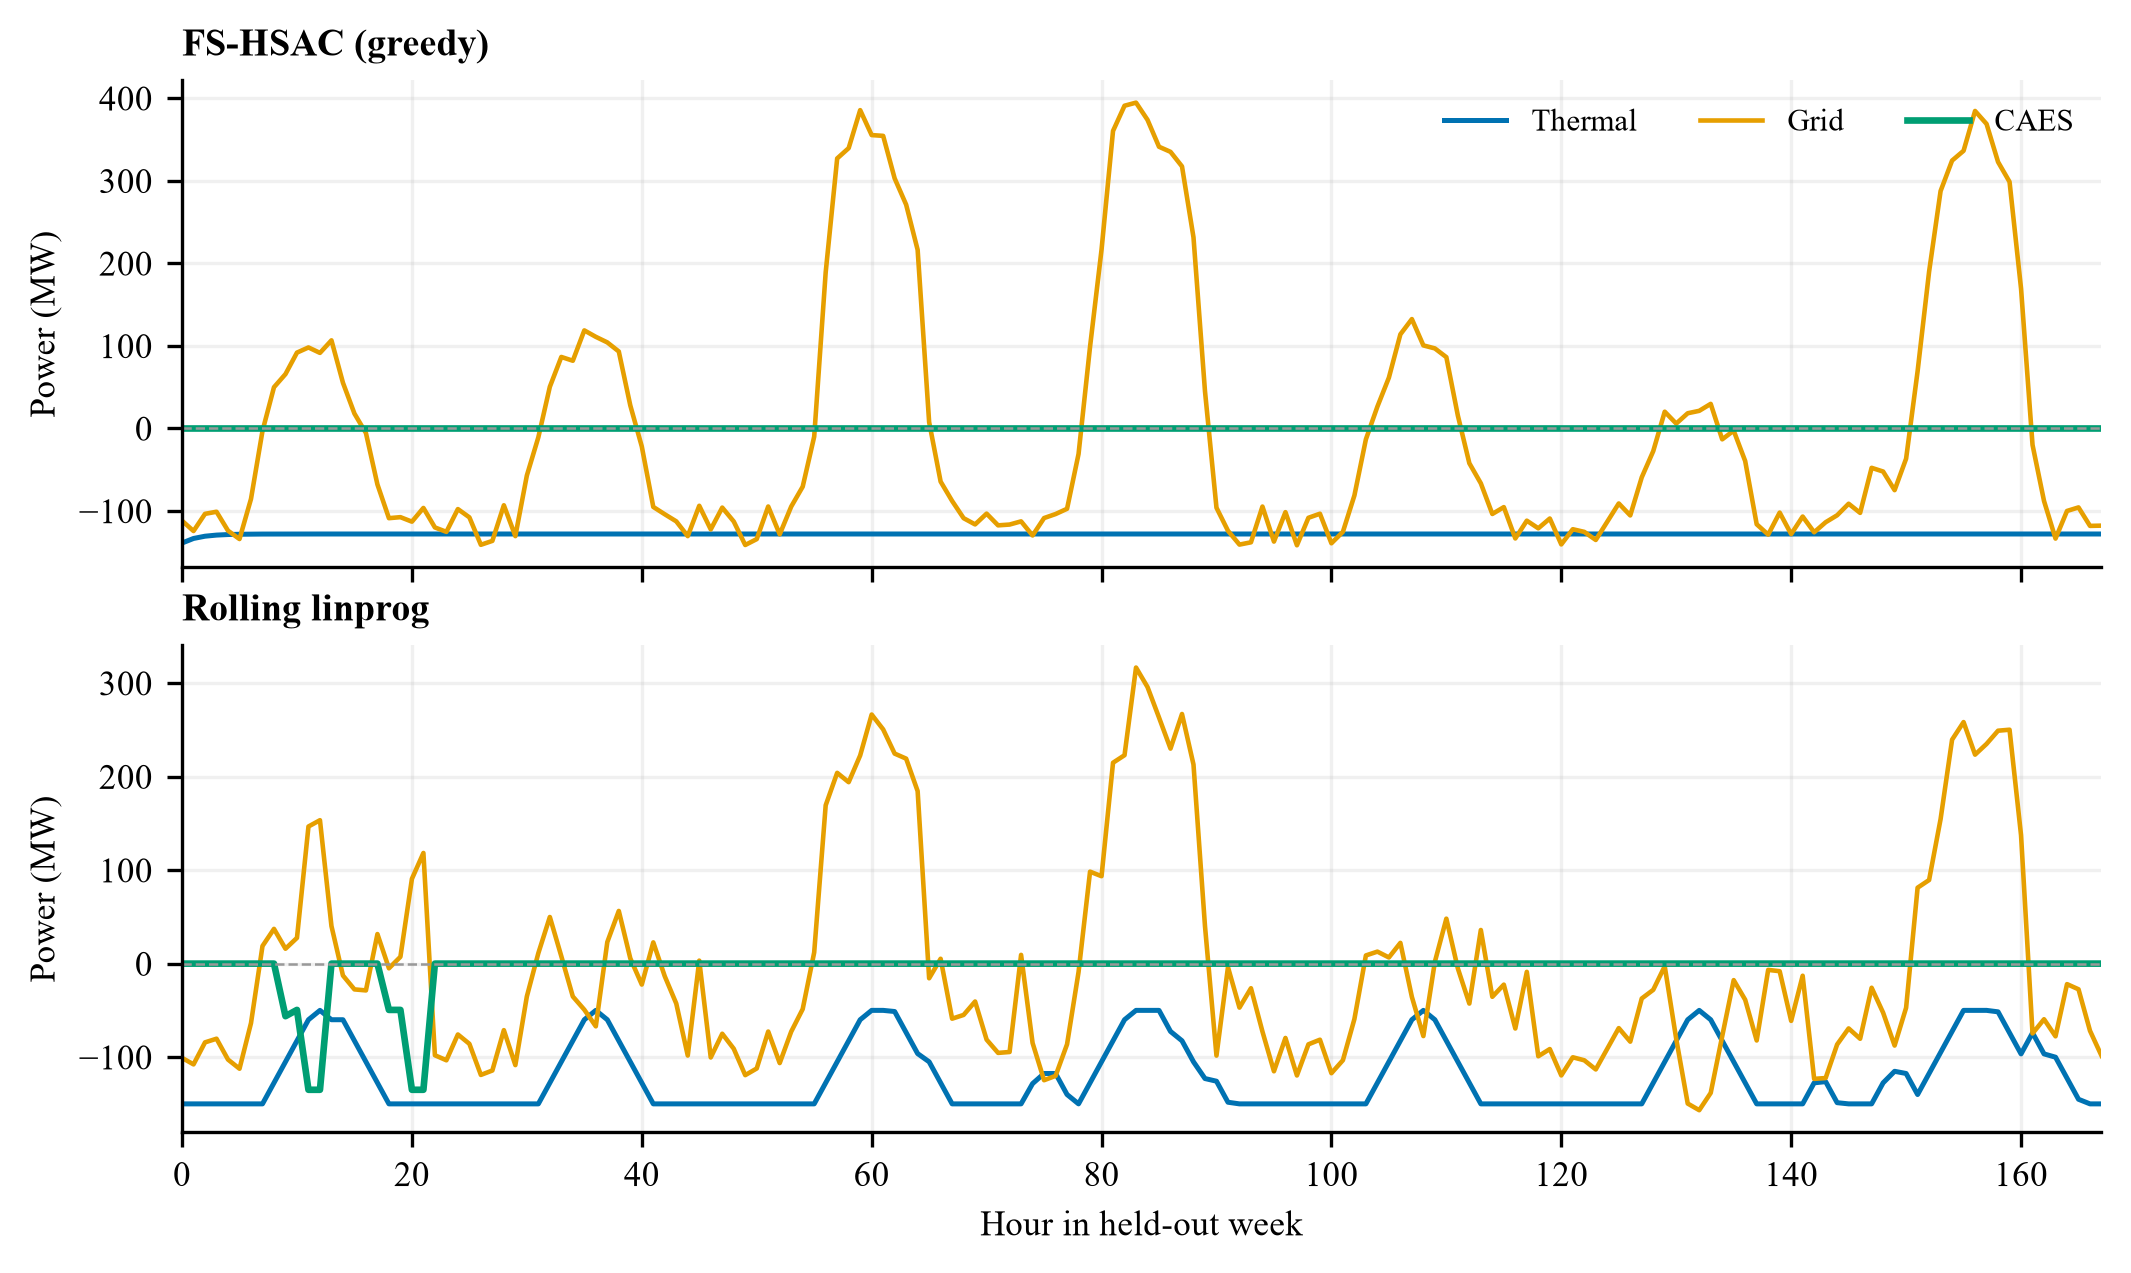
\includegraphics[width=\columnwidth,height=3.9cm,keepaspectratio]{fig_dispatch_caes}
\caption{Transition held-out week. Top: greedy FS-HSAC. Bottom: rolling linprog on the same FMU.}
\label{fig:dispatch}
\end{figure}

Projected SAC/TD3, fixed-band hybrid SAC and PSO are not in Table~\ref{tab:main}: those runs used a year-constant five-level TOU and are a different price series. The table is one seed and one held-out week per season.

\section{Conclusion}
\label{sec:conclusion}

The Sysplorer CAES DAE induces a state-dependent hybrid support \(\mathcal{A}(s)\). FS-HSAC puts a same-hour hybrid density on that support and steps the FMU through GiveSafe. Three seasonal weeks finish \(168\) hours with a reject rate below \(0.4\%\). The greedy actor leaves CAES idle; rolling linprog on the same twin uses CAES. The study is limited to one seed, weekly inventory reset, a scenario sell price, and buy levels for September--December that still follow the last published month.

\bibliographystyle{IEEEtran}
\bibliography{references}

\end{document}
